\documentclass[a4paper,11pt]{article}
\usepackage[utf8]{inputenc}
\usepackage[english]{babel}
\usepackage{graphicx}
\graphicspath{./}
\usepackage{matlab-prettifier}
\usepackage{titlesec}
\titlespacing*{\section}{0pt}{5.5ex plus 1ex minus .2ex}{4.3ex plus .2ex}
\usepackage{blindtext}
\title{ME 762: Introduction to Robotics \\ {Assignment - 2}}
\author{Devang Goyal \\ {150223}}
\date{October 10, 2018}
\usepackage[margin=0.75in]{geometry}
\begin{document}
\maketitle
\begin{section}{Matlab codes}
\begin{subsection}{Main function for catching ball}
\lstinputlisting{main_ball_catch.m}
\end{subsection}
\vspace{10 mm}
\begin{subsection}{Inverse Kinematics function}
\lstinputlisting{inverse.m}
\end{subsection}
\vspace{10 mm}
\begin{subsection}{Forward kinematics function}
\lstinputlisting{forward.m}
\end{subsection}
\end{section}
\begin{section}{Simulation}
\textbf{In this simulation ball is dropped from $(1,0,8)$ co-ordinate}\\
\textbf{Finally ball is catch ed at $(1,0,1.6928)$ co-ordinate.}\\
\vspace{10mm}
\begin{figure}[!htb]
   \begin{minipage}{0.4\textwidth}
     \centering
     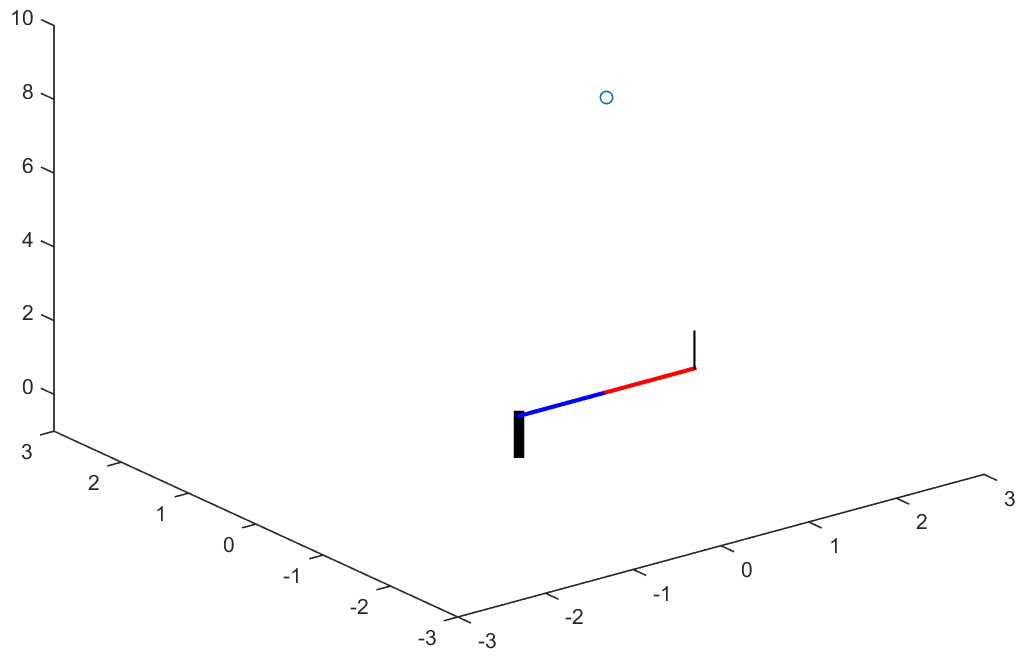
\includegraphics[width=1.25\linewidth]{FIG1.png}
   \end{minipage}\hfill
   \begin{minipage}{0.4\textwidth}
     \centering
     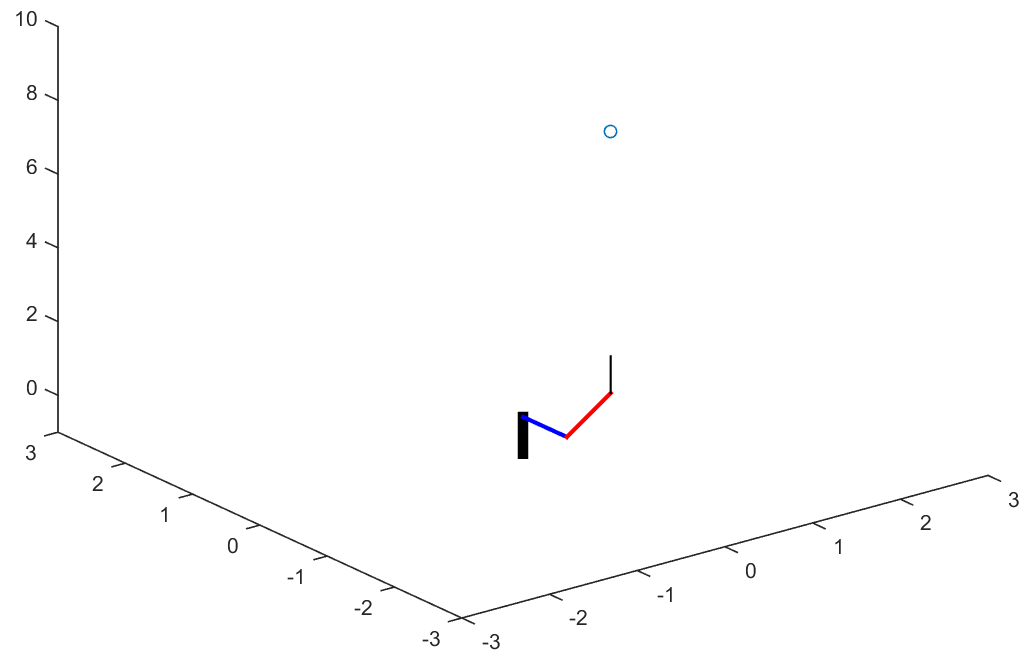
\includegraphics[width=1.25\linewidth]{FIG2.png}
   \end{minipage}
\end{figure}
\vspace{10mm}
\begin{figure}[!htb]
   \begin{minipage}{0.4\textwidth}
     \centering
     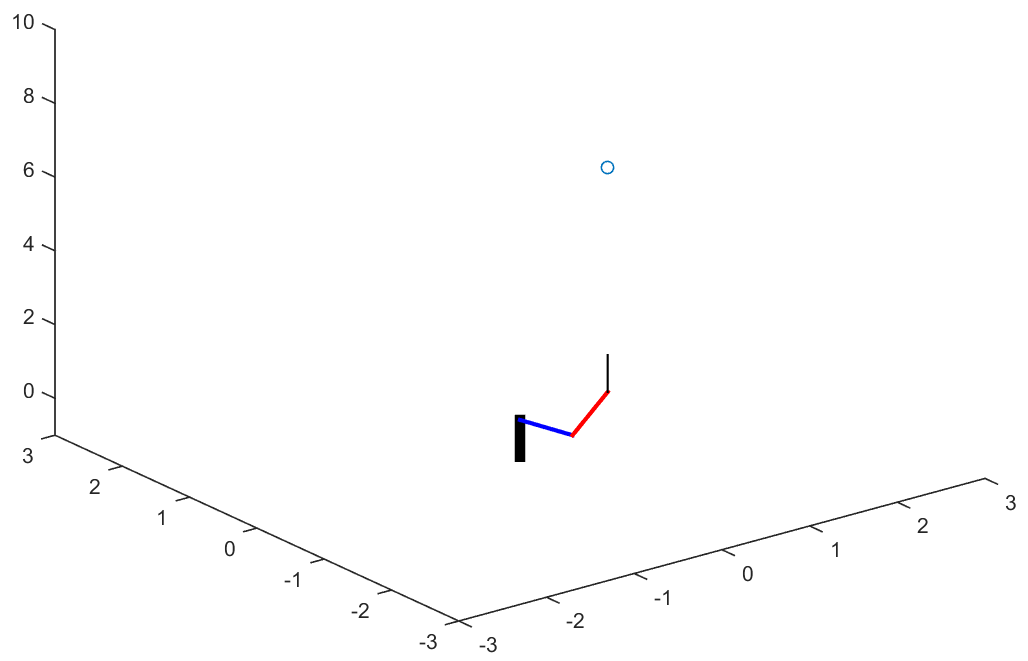
\includegraphics[width=1.25\linewidth]{FIG3.png}
   \end{minipage}\hfill
   \begin{minipage}{0.4\textwidth}
     \centering
     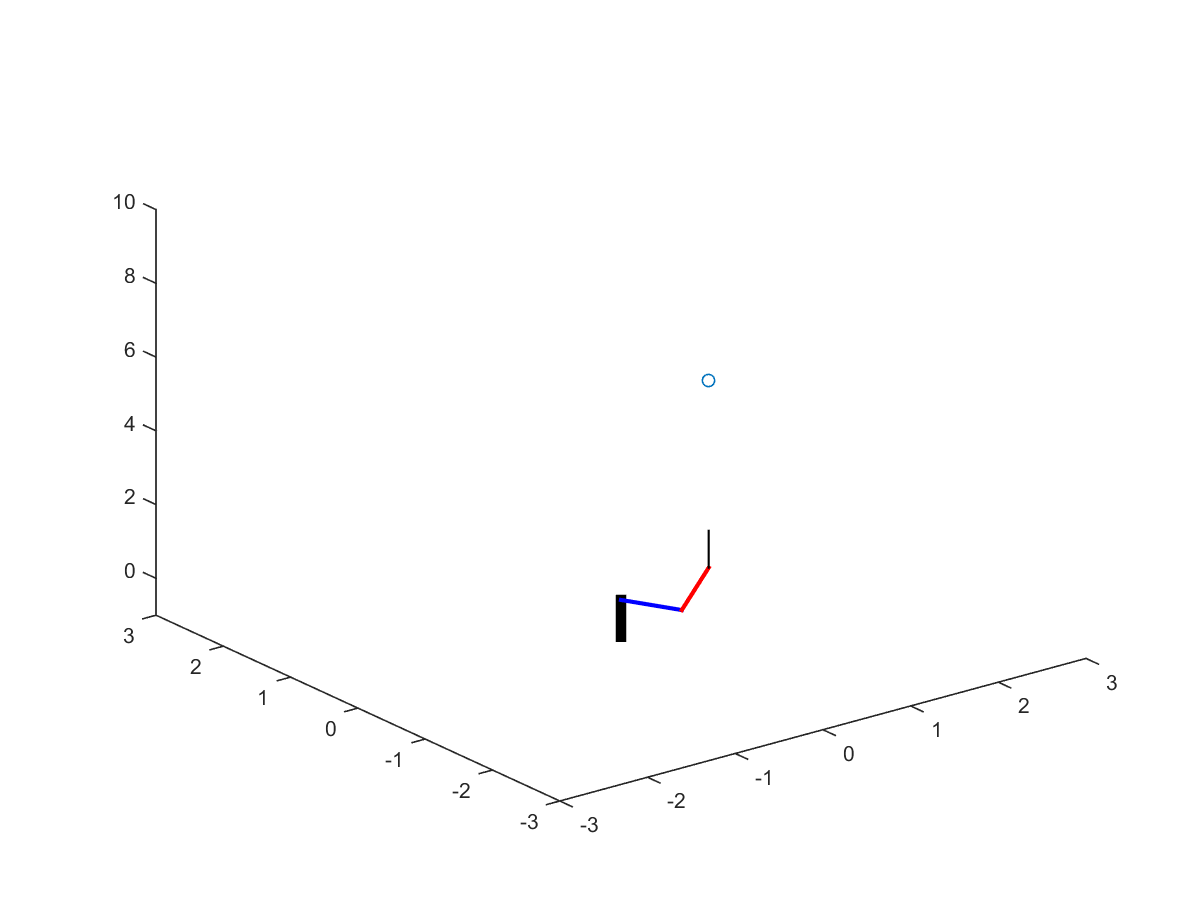
\includegraphics[width=1.25\linewidth]{FIG4.png}
   \end{minipage}
\end{figure}
\newpage
\begin{figure}[!htb]
   \begin{minipage}{0.4\textwidth}
     \centering
     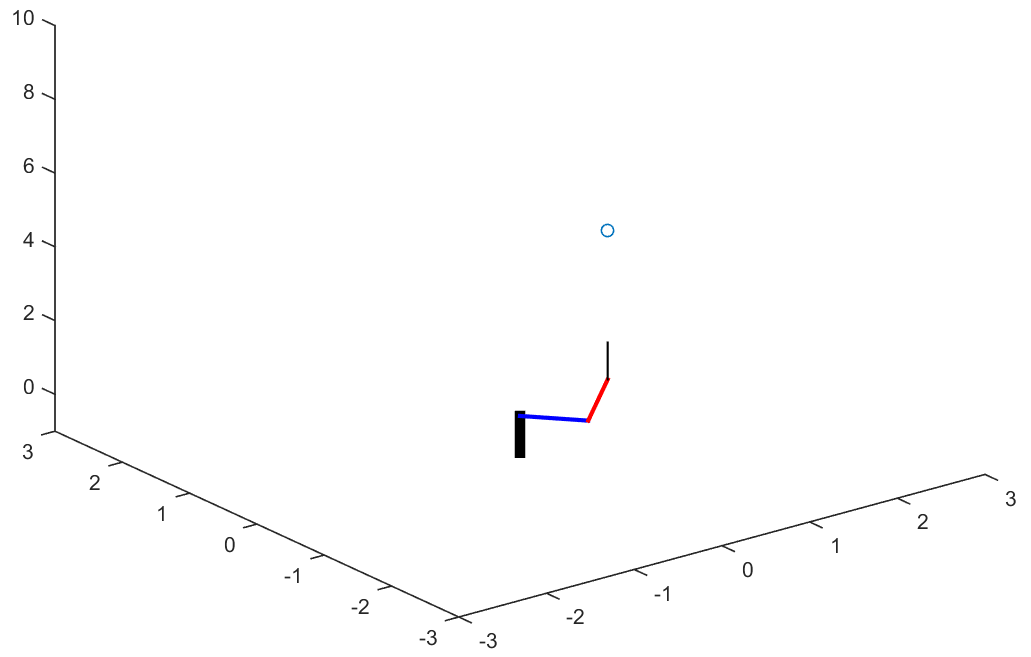
\includegraphics[width=1.25\linewidth]{FIG5.png}
   \end{minipage}\hfill
   \begin{minipage}{0.4\textwidth}
     \centering
     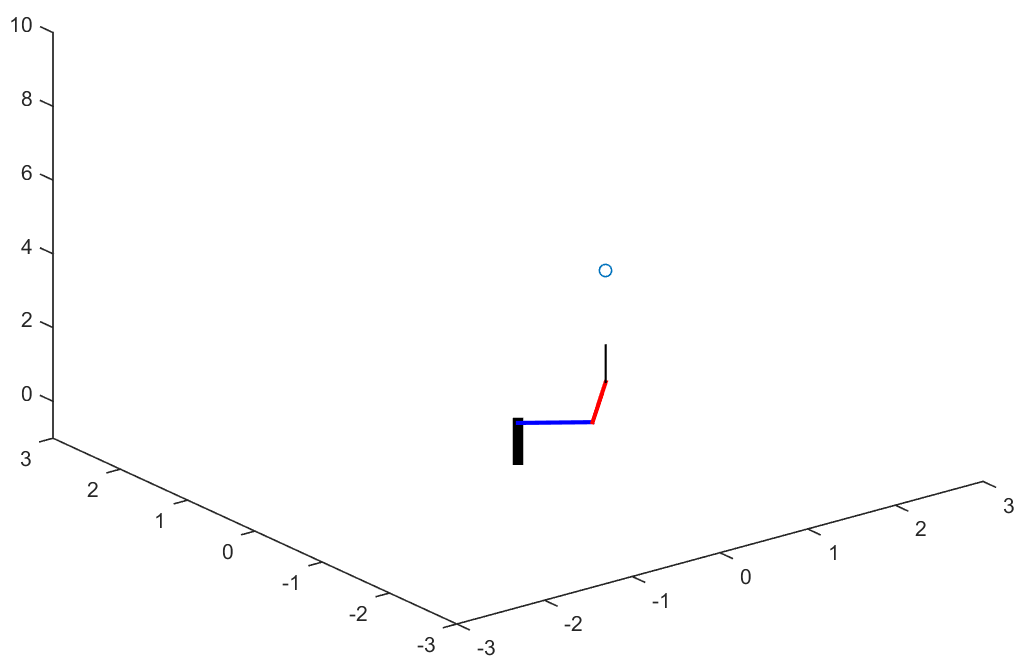
\includegraphics[width=1.25\linewidth]{FIG6.png}
   \end{minipage}
\end{figure}
\vspace{10mm}
\begin{figure}[!htb]
   \begin{minipage}{0.4\textwidth}
     \centering
     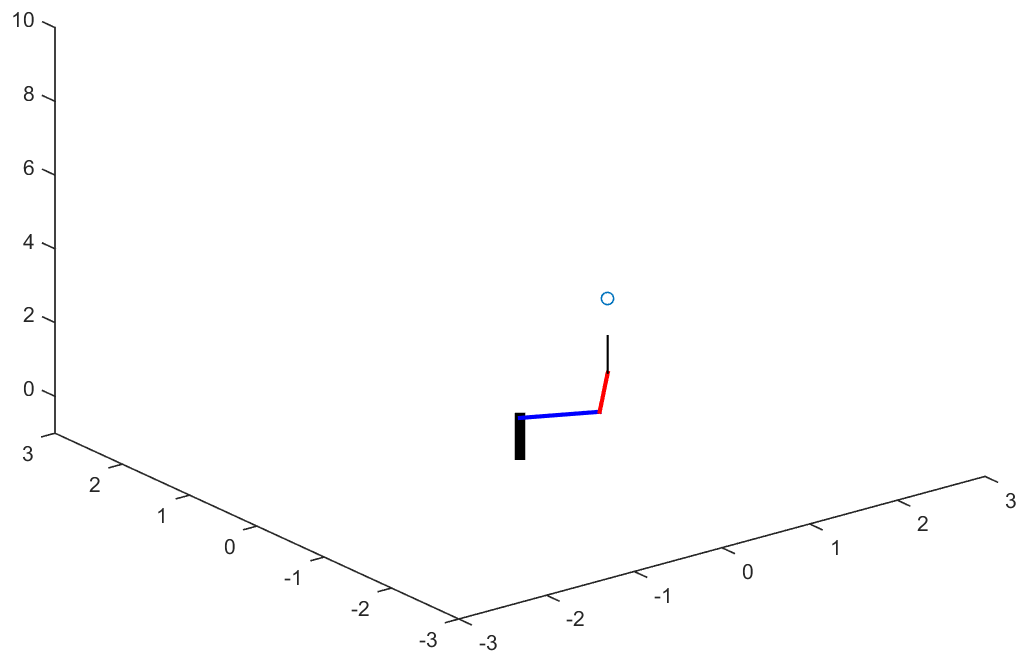
\includegraphics[width=1.25\linewidth]{FIG7.png}
   \end{minipage}\hfill
   \begin{minipage}{0.4\textwidth}
     \centering
     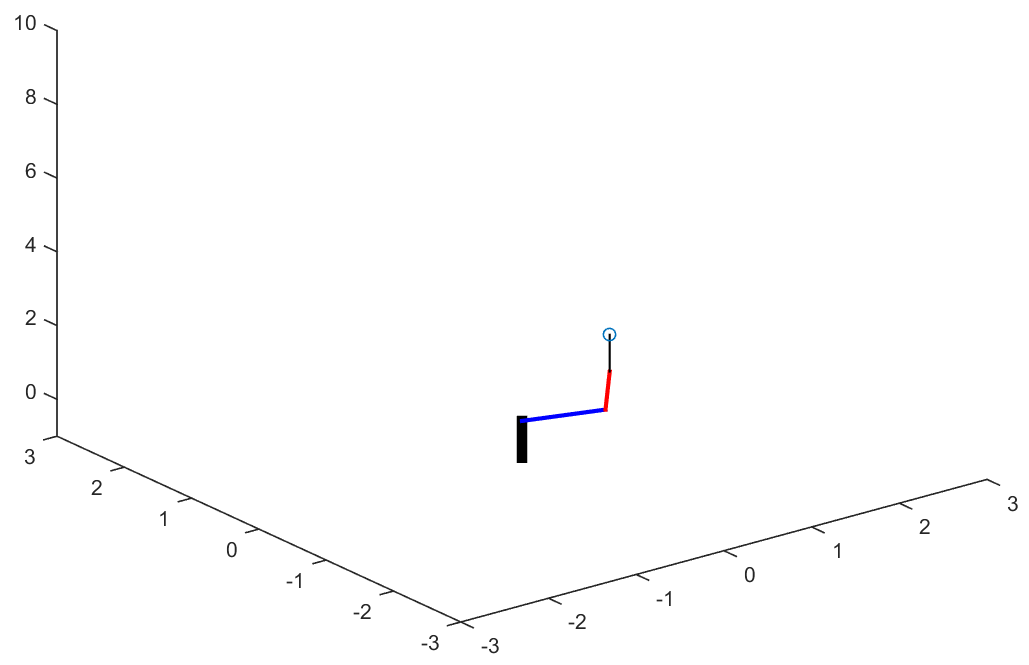
\includegraphics[width=1.25\linewidth]{FIG8.png}
   \end{minipage}
\end{figure}
\end{section}
\end{document}
